\documentclass[11pt,a4paper]{article}
\usepackage[T1]{fontenc}
\usepackage[utf8]{inputenc}
\usepackage{lmodern,microtype,amsmath,amssymb,amsthm,mathtools}
\usepackage[margin=27mm]{geometry}
\usepackage{booktabs,array,graphicx,xcolor,enumitem}
\usepackage[colorlinks=true,linkcolor=violet,citecolor=violet,urlcolor=violet]{hyperref}
\newtheorem{theorem}{Theorem}[section]
\newtheorem{lemma}[theorem]{Lemma}
\newtheorem{corollary}[theorem]{Corollary}
\newtheorem{proposition}[theorem]{Proposition}
\newtheorem{conjecture}[theorem]{Conjecture}
\theoremstyle{definition}\newtheorem{definition}[theorem]{Definition}
\theoremstyle{remark}\newtheorem{remark}[theorem]{Remark}
\newcommand{\TV}{\operatorname{TV}}
\newcommand{\E}{\mathbb E}
\newcommand{\PP}{\mathbb P}
\newcommand{\NN}{\mathbb N_0}
\newcommand{\dd}{\mathrm d}
\newcommand{\ph}{\varphi}
\DeclareMathOperator{\Mult}{Mult}
\title{Resampling heterogeneous experiments:\\ sharp amplification constants and high-signal error asymptotics}
\author{Anonymous}
\date{15 November 2026\\[2pt]\small Version 0.1.0-candidate, DOI \href{https://doi.org/10.5281/zenodo.24267748}{10.5281/zenodo.24267748}}
\begin{document}
\maketitle
\begin{abstract}
Suppose a test between two hypotheses is built from $n$ different independent experiments. One design runs each experiment once; another, called resampling or homogenisation, makes $n$ draws, each picking an experiment uniformly at random with replacement, so that some experiments are repeated and others skipped. Kontorovich proved that the second design is never more than a universal constant factor more informative than the first: $D\ge cH$ with $c>0.1489$, where $D$ and $H$ are the total-variation distances between the hypotheses under the two designs. The best published upper bound was $c\le8/9$. We show that $c\le9/14$ for experiments on general outcome spaces; already $n=2$ gives $c\le2/3$. So $8/9$, conjectured optimal for Bernoulli experiments, is not the general optimum; the Bernoulli conjecture itself is untouched. The example comes from ``erasure'' experiments, in which an observation either rules one hypothesis out or falls in a shared region whose internal distribution is the same under both. For this class we find the exact worst-case amplification $\sup H/D$ for every resampling schedule chosen independently of the data: it is $\max\{\PP(N\ne0),\max_{i,j}\E\max(N_i,N_j)\}$, where $N_i$ counts the uses of experiment $i$. For uniform resampling this is $C_n=\E\max(K,L)$, where $K$ and $L$ count the draws of two fixed experiments; it is largest at $n=3$ with value $14/9$ and, for $n\ge3$, decreasing to $1+e^{-2}(I_0(2)+I_1(2))\approx1.5238$, with $I_m$ the modified Bessel functions. For arbitrary experiments we solve the case $n=2$ exactly and give the exact bound at every distance when only two experiments differ; we also find the exact optimum for three erasure experiments. Finally, for arbitrary experiments and highly informative designs, resampling with $kn$ draws leaves overlap $1-H$ at least $q(1-D)^k$, where $q$ is the probability that every experiment is used exactly $k$ times, and this is attained to leading order as $D\to1$. For $k=1$ the optimal ratio of Bayes errors tends to $n!/n^n$. We conjecture that $9/14$ is the true general constant and report a numerical search consistent with this.
\end{abstract}

\section{Introduction}\label{sec:intro}
This section explains the problem and why it matters, records what was known, lists the new results with the class of experiments and the regime to which each applies, and gives a roadmap.

\subsection{The problem}
Two hypotheses are to be distinguished using $n$ independent experiments. Under the first hypothesis experiment $i$ produces an observation with law $P_i$; under the second, with law $Q_i$. All laws live on one measurable space. How well the hypotheses can be told apart is measured by the total variation distance
\[
\TV(P,Q)=\sup_A|P(A)-Q(A)|=\tfrac12\int|p-q|\,\dd\lambda=1-\int\min(p,q)\,\dd\lambda ,
\]
where $p,q$ are densities with respect to any dominating measure $\lambda$. With equal prior probabilities the smallest achievable error probability of a test is $(1-\TV)/2$ \cite[eq.~(1.2)]{KOct}. We call $1-\TV=\int\min(p,q)$ the \emph{overlap}; it is twice the Bayes error.

Two sampling designs are compared. The \emph{fixed design} runs each experiment once, giving
\begin{equation}\label{eq:DH}
D=\TV\Bigl(\bigotimes_{i=1}^nP_i,\ \bigotimes_{i=1}^nQ_i\Bigr).
\end{equation}
The \emph{resampled} (or homogenised) design makes $n$ draws; each draw picks an experiment uniformly at random, independently of everything else, and records only its observation. Each draw then has law $\bar P=\frac1n\sum_iP_i$ or $\bar Q=\frac1n\sum_iQ_i$, so
\[
H=\TV\bigl(\bar P^{\otimes n},\bar Q^{\otimes n}\bigr).
\]
The resampled design is the population analogue of the bootstrap and of random-design regression, and it is the kind of sampling studied in privacy amplification by subsampling \cite{BBG}. It is also analytically simpler, since $\bar P^{\otimes n}$ has identical factors \cite{KApr}. Resampling loses the guarantee that every experiment is seen once, so one might expect $H\le D$. That is false: $H$ can exceed $D$ \cite{KJan}. The question is by how much.

\subsection{What was known}
Kontorovich showed that resampling cannot help much: there is a universal constant $c>0$, independent of $n$ and of the outcome space, such that
\begin{equation}\label{eq:homog}
D\ge c\,H .
\end{equation}
This was first proved for Bernoulli experiments \cite{KJan} and then for arbitrary probability measures, with $c>0.1489$ \cite{KApr}. A later local-to-global theorem treats general $f$-divergences \cite{KOct}; for total variation its Section~7.3 gives, in the language of likelihood-ratio laws, the bound $H\le\frac32D$ for $n=2$. In the other direction, Kontorovich's Bernoulli example shows $c\le8/9$. The April paper records that this bound holds ``a fortiori in general'' and that $8/9$ ``was conjectured to be optimal'' \cite[p.~1]{KApr}; the conjecture itself is stated for Bernoulli products, that is, for a common two-point outcome space \cite[remarks after Theorem~1.5]{KJan}. The sharp value of $c$ was open in both settings.

\subsection{What is new}
Write $c^*$ for the best constant in \eqref{eq:homog} over arbitrary measurable spaces.
\begin{enumerate}[leftmargin=*]
\item \textbf{A better obstruction for the general constant (Section~\ref{sec:uniform}).} $c^*\le 9/14\approx0.643$. The case $n=2$ already gives $c^*\le2/3$, and every $n\ge3$ gives $c^*<0.6563$. Hence $8/9$ is not the optimal general constant. The examples use at least three outcome symbols and do not bear on the Bernoulli conjecture.
\item \textbf{Exact amplification for erasure experiments under any schedule (Sections~\ref{sec:setup}--\ref{sec:uniform}).} An \emph{erasure experiment} is one whose likelihood ratio takes at most one value in $(0,\infty)$: each observation either rules one hypothesis out or lands in a shared region, which the two hypotheses may reach with different probabilities but within which they behave identically. For such experiments and every revealed resampling schedule independent of the data, $\sup H/D=\max\{\PP(N\ne0),\max_{i,j}\E\max(N_i,N_j)\}$ (Theorem~\ref{thm:schedule}). For uniform resampling this is $C_n=\E\max(K,L)$, maximal at $n=3$ with value $14/9$, and $C_n\downarrow 1+e^{-2}(I_0(2)+I_1(2))$ (Theorem~\ref{thm:uniform}, Proposition~\ref{prop:limit}).
\item \textbf{Arbitrary experiments with two differing coordinates (Section~\ref{sec:two}).} If $P_i=Q_i$ except in two coordinates, the exact bound is $H\le F_n(D)$ with an explicit polynomial $F_n$, attained at every $D$. In particular the unrestricted problem for $n=2$ is solved: $\sup H=\frac32D-\frac12D^2$ (Corollary~\ref{cor:n2}).
\item \textbf{Three erasure experiments at every distance (Section~\ref{sec:three}).} The exact optimum, with two phase transitions and algebraic optimisers.
\item \textbf{Arbitrary experiments, high signal (Section~\ref{sec:strongall}).} For any data-independent schedule with $kn$ draws, the optimal overlap is $q\,(1-D)^k$ to leading order as $D\to1$, where $q$ is the probability that every experiment is used exactly $k$ times. The lower bound $1-H\ge q(1-D)^k$ holds at every distance; the leading term is attained, with an explicit power-saving remainder. For uniform resampling with $k=1$ the optimal ratio of Bayes errors tends to $n!/n^n$.
\end{enumerate}
Section~\ref{sec:discussion} states the conjecture $c^*=9/14$ and reports a numerical search over arbitrary finite experiments that found no ratio above $C_n$.

The erasure class is a genuine restriction. Section~\ref{sec:discussion} shows that an informative experiment with mutually absolutely continuous laws cannot be garbled into an erasure experiment, so the constants in items~2 and~4 are not known to bound general experiments. Items~1, 3 and~5 hold for arbitrary experiments.

\subsection{Relation to other work}
The labelled lifting used in Section~\ref{sec:setup}, which records which experiment produced each observation, is Kontorovich's device \cite[Theorem~3 and proof of Theorem~4]{KApr}, \cite[Proposition~5.3]{KOct}. The coefficient $n!/n^n$ in item~5 is the classical probability that $n$ draws with replacement from $n$ objects are all distinct; equivalently, one minus the total variation between sampling with and without replacement \cite[p.~198, eq.~(1)]{Sampling}. What is new is that this coefficient is attained simultaneously over all other count patterns. Privacy amplification by subsampling studies the same resampling designs with the hockey-stick divergence; at privacy parameter $\varepsilon=0$ that divergence is total variation, and the multinomial bound of \cite[Theorem~10]{BBG}, which handles one differing record through group privacy, is a one-coordinate counterpart of Theorems~\ref{thm:schedule} and~\ref{thm:twoactive}. We did not find the schedule constant, the two-coordinate modulus, the three-component optimum or the high-signal attainment theorem in these sources. Standard tensorisation facts for total variation are in \cite{KTen}.

\subsection{Roadmap}
Section~\ref{sec:setup} defines erasure experiments, schedules and the labelled lift. Section~\ref{sec:schedule} proves the exact schedule constant. Section~\ref{sec:uniform} specialises to uniform resampling and derives $c^*\le9/14$. Section~\ref{sec:two} treats arbitrary experiments with two differing coordinates and solves $n=2$. Section~\ref{sec:three} gives the full three-component erasure optimum. Section~\ref{sec:strongall} proves the high-signal theorem for arbitrary experiments. Section~\ref{sec:discussion} interprets the results, states the conjecture with numerical evidence, and lists open problems.

\section{Erasure experiments, schedules and labels}\label{sec:setup}
This section fixes the class of erasure experiments, the random schedules that generalise uniform resampling, and the labelled experiment that later proofs work with.

\begin{definition}\label{def:class}
A pair $(P_i,Q_i)$ is an \emph{erasure experiment} if, for some $r_i,s_i\in[0,1]$,
\begin{equation}\label{eq:erasure}
 P_i=r_iR_i+(1-r_i)S_i,\qquad
 Q_i=s_iR_i+(1-s_i)T_i,
\end{equation}
where $R_i,S_i,T_i$ are mutually singular probability measures (a component with zero coefficient can be omitted). We call $r_i,s_i$ the \emph{common masses}.
\end{definition}
The three disjoint regions carry probabilities $(r_i,1-r_i,0)$ under $P_i$ and $(s_i,0,1-s_i)$ under $Q_i$, and inside each region the conditional law does not depend on the hypothesis. Equivalently, the likelihood ratio $\dd P_i/\dd Q_i$ takes at most one value in $(0,\infty)$, namely $r_i/s_i$ on the common region, besides $0$ and $\infty$. For testing purposes the experiment is the output of a binary-input channel with three outputs, ``common'', ``rules out $Q$'' and ``rules out $P$''; the symmetric case $r_i=s_i$ is the classical erasure channel. Arbitrary Bernoulli pairs are not erasure experiments.

For a product of erasure experiments the common part is exactly the product of the common regions, on which the two product densities are constant multiples of one another; elsewhere one of them vanishes. Hence
\begin{equation}\label{eq:overlap}
1-D=\min\Bigl\{\prod_i r_i,\ \prod_i s_i\Bigr\}.
\end{equation}
When $D<1$ every $r_i$ and $s_i$ is positive, and we put
\begin{equation}\label{eq:logs}
a_i=-\log r_i,\quad b_i=-\log s_i,\quad
M=\max\Bigl\{\sum_i a_i,\sum_i b_i\Bigr\}=-\log(1-D),\qquad
\ph(t)=1-e^{-t},
\end{equation}
so that $D=\ph(M)$. We call $a_i,b_i$ the \emph{logarithmic budgets}.

\paragraph{Schedules.} Let $N=(N_1,\ldots,N_n)\in\NN^n$ be random with a fixed law $\nu$, independent of the hypothesis and of all observations, and with $\E\sum_iN_i<\infty$. The coordinates of $N$ may be dependent. The \emph{scheduled experiment} reveals $N$ and then takes $N_i$ independent observations from pair $i$; its outcome space is the disjoint union of the corresponding product spaces. Write $H_\nu$ for the total variation between its two laws. Conditioning on the revealed schedule gives, for erasure experiments,
\begin{equation}\label{eq:schedule}
H_\nu=1-\E\min\Bigl\{\prod_i r_i^{N_i},\ \prod_i s_i^{N_i}\Bigr\}\qquad(0^0:=1),
\end{equation}
and an empty product carries no information. When $D<1$ this reads
\[
H_\nu=\E\,\ph\bigl(\max\{N\cdot a,N\cdot b\}\bigr).
\]

\paragraph{The labelled lift.} Uniform resampling corresponds to counts $N$ with the multinomial law $\Mult(n;1/n,\ldots,1/n)$. The resampled experiment of Section~\ref{sec:intro} records only the observations; recording also the sequence of sampled indices gives a \emph{labelled} experiment. Given the counts, the order of the indices is independent of the hypothesis, and given the index sequence the observations form a product that differs from the count-conditional product only by a permutation of coordinates; so the labelled experiment has total variation $H_\nu$. Forgetting the labels is a measurable map, which cannot increase total variation, so $H\le H_\nu$. This lifting argument is Kontorovich's \cite[Theorem~3 and proof of Theorem~4]{KApr}, \cite[Proposition~5.3]{KOct}. If every observation that can occur under both hypotheses reveals its index, forgetting labels loses nothing and $H=H_\nu$; this is checked for each extremal example below.

\section{The exact constant for every independent schedule}\label{sec:schedule}
This section proves the main structural fact for erasure experiments: the worst-case linear amplification under a schedule depends only on the chance of an empty schedule and on the pairwise laws of the counts.

\begin{theorem}[Sharp schedule constant]\label{thm:schedule}
For a schedule $\nu$ as in Section~\ref{sec:setup}, put
\begin{equation}\label{eq:K}
p_\nu=\PP(N\ne0),\qquad
C_\nu=\max_{1\le i,j\le n}\E\max(N_i,N_j),\qquad
\kappa_\nu=\max\{p_\nu,C_\nu\}.
\end{equation}
Over all finite families of erasure experiments with $D>0$, the supremum of $H_\nu/D$ equals $\kappa_\nu$; it is approached but in general not attained. If $p_\nu>0$, the stronger nonlinear bound
\begin{equation}\label{eq:jensen}
H_\nu\le p_\nu\left[1-(1-D)^{C_\nu/p_\nu}\right]\le \kappa_\nu D
\end{equation}
holds; it is not claimed to be sharp. If $p_\nu=0$ then $H_\nu=0$. Both bounds also hold for any experiment obtained by forgetting part of the observations, in particular for uniform resampling without labels.
\end{theorem}
\begin{proof}
If $p_\nu=0$ then $N=0$ almost surely and $H_\nu=0$. Assume $p_\nu>0$ and first $0<D<1$, so that the logarithmic budgets are finite. They lie in the product of simplices
\[
\mathcal S_M\times\mathcal S_M,\qquad
\mathcal S_M=\Bigl\{x\in[0,\infty)^n:\ \textstyle\sum_i x_i\le M\Bigr\}.
\]
The function $G(a,b)=\E\max\{N\cdot a,N\cdot b\}$ is finite and convex on this set. Every point is a convex combination of vertex pairs, so $G$ is at most its largest value at a pair of vertices. The vertices of $\mathcal S_M$ are $0,Me_1,\ldots,Me_n$; the pair $(Me_i,Me_j)$ gives $M\E\max(N_i,N_j)$ (for $i=j$ this is $M\E N_i$), and a pair containing the zero vertex gives no more. Thus
\begin{equation}\label{eq:simplex}
G(a,b)\le MC_\nu.
\end{equation}
Since $\ph$ is increasing and concave with $\ph(0)=0$, Jensen's inequality conditional on $\{N\ne0\}$ gives
\[
H_\nu\le p_\nu\,\ph\!\left(\frac{G(a,b)}{p_\nu}\right)
       \le p_\nu\,\ph\!\left(\frac{MC_\nu}{p_\nu}\right).
\]
For $\lambda\ge1$, concavity and $\ph(0)=0$ give $\ph(\lambda M)\le\lambda\ph(M)$; for $0\le\lambda\le1$, monotonicity gives $\ph(\lambda M)\le\ph(M)$. With $\lambda=C_\nu/p_\nu$ this proves \eqref{eq:jensen}. If $D=0$ all pairs coincide; if $D=1$ then $H_\nu\le p_\nu\le\kappa_\nu$. The final assertion holds because a measurable map cannot increase total variation.

\emph{Sharpness of $C_\nu$.} Take a maximising pair $i\ne j$. Give coordinate $i$ common masses $(r_i,s_i)=(1,1-d)$, coordinate $j$ common masses $(1-d,1)$, and make all other pairs identical. Then $D=d$ by \eqref{eq:overlap}, and by \eqref{eq:schedule}
\begin{equation}\label{eq:exactpair}
H_\nu=\E\left[1-(1-d)^{\max(N_i,N_j)}\right].
\end{equation}
For every integer $m\ge0$, $[1-(1-d)^m]/d\le m$ and the ratio tends to $m$ as $d\downarrow0$; dominated convergence gives $H_\nu/d\to\E\max(N_i,N_j)$. If the maximising indices coincide, the single one-sided pair $(1,1-d)$ in coordinate $i$ gives the limit $\E N_i$.

\emph{Sharpness of $p_\nu$.} Take $r_i=s_i=e^{-M/n}$ for all $i$. Then $D=1-e^{-M}$ and
$H_\nu=\E[1-e^{-M\sum_iN_i/n}]\to p_\nu$ as $M\to\infty$, while $D\to1$.
\end{proof}

\begin{remark}
The schedule must be independent of the observations and the hypothesis; adaptive schedules are not covered. The counts themselves may be dependent.
\end{remark}

\subsection{Examples: the count law matters, not just the mean}
The constant separates schedules with the same expected use $\E N_i$ of every experiment. All observations and labels are retained.
\begin{center}
\begin{tabular}{p{0.66\textwidth}c}
\toprule
Schedule & Sharp factor $\kappa_\nu$\\
\midrule
With probability $\theta$ use every experiment once, otherwise observe nothing & $\theta$\\[3pt]
Use a random set of experiments of fixed nonzero size, each at most once & $1$\\[3pt]
Choose one experiment uniformly and repeat it $m\ge1$ times ($n\ge2$) & $\max\{1,2m/n\}$\\
\bottomrule
\end{tabular}
\end{center}
In the first row $H_\nu=\theta D$ for arbitrary experiments. In the second every count is at most one, so $C_\nu\le p_\nu=1$. In the third, distinct indices give $\E\max(N_i,N_j)=2m/n$. Choosing one experiment and repeating it $n$ times therefore has factor $2$, whereas choosing afresh for each of $n$ draws has factor at most $14/9$ (next section), although both designs use each experiment once on average.

\section{Uniform resampling and the obstruction \texorpdfstring{$c^*\le 9/14$}{c* <= 9/14}}\label{sec:uniform}
This section evaluates the schedule constant for uniform resampling, shows that it peaks at $n=3$, computes its limit, and turns the extremal example into the bound $c^*\le9/14$ for arbitrary experiments.

For $n\ge2$ let $(K,L,n-K-L)\sim\Mult(n;1/n,1/n,1-2/n)$, the numbers of draws that pick two fixed experiments, and define
\begin{equation}\label{eq:Cn}
 C_n=\E\max(K,L)=1+\tfrac12\E|K-L|.
\end{equation}
\begin{theorem}\label{thm:uniform}
For $n\ge2$ erasure experiments, $H\le C_nD$, and $C_n$ is sharp (as $D\to0$) when arbitrary outcome spaces are allowed. Moreover $C_2=3/2$, $C_3=14/9$, and $C_n$ strictly decreases for $n\ge3$. Consequently $H\le\frac{14}{9}D$ is the sharp dimension-free inequality for erasure experiments, and the best constant in \eqref{eq:homog} for arbitrary experiments satisfies
\begin{equation}\label{eq:fourteen}
c^*\le \frac{9}{14}.
\end{equation}
\end{theorem}
\begin{proof}
Theorem~\ref{thm:schedule} applies with $p_\nu=1$. By exchangeability every pair of distinct indices gives the same expectation, and $\E N_i=1\le C_n$, so the factor is $C_n$. To compare different $n$, write $Z_n=K-L$, whose characteristic function is
\[
\E e^{itZ_n}=\left(1-\frac{2(1-\cos t)}n\right)^n.
\]
The identity
\[
|m|=\frac1\pi\int_0^\pi\frac{1-\cos(mt)}{1-\cos t}\,\dd t\qquad(m\in\mathbb Z)
\]
therefore gives
\begin{equation}\label{eq:absfourier}
\E|Z_n|=\frac1\pi\int_0^\pi
\frac{1-[1-x(t)/n]^n}{1-\cos t}\,\dd t,\qquad x(t)=2(1-\cos t)\in[0,4].
\end{equation}
For fixed $x>0$ and real $u>x$, the function $(1-x/u)^u$ strictly increases with $u$: its logarithmic derivative is $\log(1-v)+v/(1-v)$ with $v=x/u\in(0,1)$, which vanishes at $v=0$ and has derivative $v/(1-v)^2>0$. This gives the pointwise ordering for successive integers $n\ge4$, with the endpoint $x=4,n=4$ by continuity. For $n=3$ against $4$ the same argument works when $x<3$; when $3\le x\le4$ the cube $(1-x/3)^3$ is nonpositive and the fourth power is nonnegative. The ordering is strict for almost every $t\in(0,\pi)$, so \eqref{eq:absfourier} gives strict decrease from $n=3$ on. Direct enumeration gives $\E|Z_2|=1$ and $\E|Z_3|=10/9$. Sharpness, for the unlabelled experiment, and \eqref{eq:fourteen} follow from the explicit family in Section~\ref{sec:five}.
\end{proof}

\begin{proposition}[The large-$n$ limit]\label{prop:limit}
As $n\to\infty$,
\[
C_n\downarrow C_\infty:=\E\max(X,Y)=1+e^{-2}\bigl(I_0(2)+I_1(2)\bigr)\approx1.5237776,
\]
where $X,Y$ are independent Poisson variables with mean $1$ and $I_m$ is the modified Bessel function of the first kind. Hence $C_n>C_\infty>3/2$ for all $n\ge3$, and every $n\ge3$ gives the obstruction $c^*\le1/C_n<1/C_\infty\approx0.6563$.
\end{proposition}
\begin{proof}
The multinomial probabilities $\PP(K=a,L=b)$ converge to $e^{-2}/(a!\,b!)$, so $(K,L)\to(X,Y)$ in distribution. Since $\max(K,L)^2\le(K+L)^2$ and $\E(K+L)^2=2(1-2/n)+4\le6$, the variables $\max(K,L)$ are uniformly integrable and $C_n\to\E\max(X,Y)=1+\frac12\E|X-Y|$. For $m\ge0$, $\PP(X-Y=m)=e^{-2}\sum_{j\ge0}1/(j!\,(j+m)!)=e^{-2}I_m(2)$, and the law of $X-Y$ is symmetric. The recurrence $I_{m-1}(z)-I_{m+1}(z)=(2m/z)I_m(z)$ at $z=2$ gives $mI_m(2)=I_{m-1}(2)-I_{m+1}(2)$, so $\sum_{m\ge1}mI_m(2)$ telescopes to $I_0(2)+I_1(2)$. Hence $\E|X-Y|=2e^{-2}(I_0(2)+I_1(2))$. With the strict decrease in Theorem~\ref{thm:uniform}, $C_n>C_\infty$ for $n\ge3$.
\end{proof}

\subsection{A five-outcome extremal family}\label{sec:five}
For $n\ge3$ take outcomes $a_0,a_1,b_0,b_1,c$ and set, for $0<d\le1$,
\begin{align}\label{eq:five}
P_1&=\delta_{a_0},& Q_1&=(1-d)\delta_{a_0}+d\delta_{a_1},\notag\\
P_2&=(1-d)\delta_{b_0}+d\delta_{b_1},& Q_2&=\delta_{b_0},\\
P_i&=Q_i=\delta_c&& (3\le i\le n).\notag
\end{align}
For $n=2$ omit the neutral outcome $c$. The fixed-design overlap is $1-d$, so $D=d$. The neutral observations are identical under both hypotheses and every other observation reveals its index, so $H=H_\nu$; the numbers of $a$- and $b$-observations have the law of $(K,L)$, and the conditional overlap is $(1-d)^{\max(K,L)}$. Hence
\begin{equation}\label{eq:Fn}
 H=F_n(d):=\E\left[1-(1-d)^{\max(K,L)}\right],\qquad
 \lim_{d\downarrow0}\frac{F_n(d)}d=C_n,
\end{equation}
and in particular
\begin{equation}\label{eq:F2F3}
F_2(d)=\frac32d-\frac12d^2,\qquad
F_3(d)=\frac{14}{9}d-\frac23d^2+\frac{2}{27}d^3.
\end{equation}
At $d=1/10$ the $n=3$ family gives $H=2011/13500$ and $D/H=1350/2011<8/9$. These experiments need distinct symbols across components. Realised on a single two-point space, the first two pairs become $\mathrm{Ber}(1)$ against $\mathrm{Ber}(1-d)$ and $\mathrm{Ber}(1-d)$ against $\mathrm{Ber}(1)$; the informative symbol of one coordinate then coincides with the common symbol of the other, $\bar P=\bar Q$ and $H=0$. So the family says nothing about the Bernoulli conjecture.

\begin{remark}[Consequence for proofs through labels]\label{rem:labelled}
The proof in \cite{KApr} passes through the labelled experiment and then forgets labels. The family above has $H_\nu/D\to14/9$, so any argument that bounds the labelled distance $H_\nu$ by $D/c$ must have $c\le9/14$. The same holds on a two-point space: realised there, the first two pairs of \eqref{eq:five} are Bernoulli pairs whose labelled ratio still tends to $14/9>9/8$, although their unlabelled $H$ vanishes. So a proof of the Bernoulli conjecture $c=8/9$ \cite{KJan} would have to use the loss of labels.
\end{remark}

\section{Arbitrary experiments with two differing coordinates}\label{sec:two}
This section drops the erasure restriction but assumes that at most two experiments differ between the hypotheses. It gives the exact bound at every distance for every schedule and, as a consequence, solves the unrestricted problem for $n=2$.

\begin{theorem}\label{thm:twoactive}
Suppose $n\ge2$ and $P_i=Q_i$ for all $i\ge3$, with $(P_1,Q_1)$ and $(P_2,Q_2)$ arbitrary. For every schedule as in Section~\ref{sec:setup},
\begin{equation}\label{eq:two-schedule}
H_\nu\le\E\left[1-(1-D)^{\max(N_1,N_2)}\right],
\end{equation}
and this bound is attained for each $D\in[0,1]$ (a zero count contributes zero, also at $D=1$). For uniform resampling, $H\le F_n(D)$, attained for every $D$. For $0<D\le1$, $F_n(D)$ strictly decreases in $n\ge3$, so the exact envelope over all $n\ge2$ is
\begin{equation}\label{eq:envelope}
\max\{F_2(D),F_3(D)\}=
\begin{cases}
F_3(D),&0\le D\le D_*,\\
F_2(D),&D_*\le D\le1,
\end{cases}
\qquad D_* =\frac{9-\sqrt{33}}8\approx0.4069.
\end{equation}
\end{theorem}
\begin{proof}
Fix counts $(k,l)$ for the two differing coordinates. Group the conditional experiment into $\min(k,l)$ copies of the pair $(P_1\otimes P_2,Q_1\otimes Q_2)$ and $|k-l|$ copies of a single coordinate. Each group has total variation at most $D$: the first kind equals $D$ because the remaining coordinates are identical, and the second is at most $D$ by marginal contraction. Integrating $\min(\prod_j u_j,\prod_j v_j)\ge\prod_j\min(u_j,v_j)$ gives the product-overlap inequality
\[
1-\TV\Bigl(\bigotimes_j U_j,\bigotimes_j V_j\Bigr)
\ge\prod_j\bigl[1-\TV(U_j,V_j)\bigr],
\]
so the conditional total variation is at most $1-(1-D)^{\max(k,l)}$. Averaging over the schedule gives \eqref{eq:two-schedule}; for uniform sampling the right side is $F_n(D)$, and forgetting labels preserves the bound. Family~\eqref{eq:five} attains equality in every count case, so both bounds are exact.

For monotonicity put $\tau=\sqrt{1-D}$ and first assume $0<\tau<1$. The Poisson kernel
$P_\tau(t)=(1-\tau^2)/(1-2\tau\cos t+\tau^2)$ is positive and has Fourier coefficients $\tau^{|m|}$. Since $2\max(K,L)=K+L+|K-L|$ and $\E\,\tau^{K+L}e^{it(K-L)}=[1-2(1-\tau\cos t)/n]^n$,
\begin{equation}\label{eq:poisson}
1-F_n(D)=\frac1{2\pi}\int_{-\pi}^{\pi}P_\tau(t)
\left[1-\frac{2(1-\tau\cos t)}n\right]^n\dd t.
\end{equation}
Here $2(1-\tau\cos t)\in(0,4)$, so the pointwise ordering from Theorem~\ref{thm:uniform} shows that the overlap $1-F_n(D)$ strictly increases with $n\ge3$. At $D=1$ use $\tau=0$ in the same formula. Finally $F_3(D)-F_2(D)=\frac{D}{54}(4D^2-9D+3)$, which gives \eqref{eq:envelope}; $D=0$ is equality throughout.
\end{proof}

\begin{corollary}[The case $n=2$ is solved]\label{cor:n2}
For two arbitrary pairs of probability measures on any measurable space,
\[
H\le\frac32D-\frac12D^2,\qquad\text{equivalently}\qquad 1-H\ge\frac{(1-D)(2-D)}2 ,
\]
with equality for every $D\in[0,1]$ in family~\eqref{eq:five}. In particular the best constant in \eqref{eq:homog} restricted to $n=2$ is exactly $2/3$, and for $0\le D<1$ the ratio of resampled to fixed-design Bayes errors is at least $(2-D)/2$, which tends to $1/2$ as $D\uparrow1$.
\end{corollary}
\begin{proof}
For $n=2$ the hypothesis $P_i=Q_i$ for $i\ge3$ is vacuous, so Theorem~\ref{thm:twoactive} applies to all experiments, and $F_2$ is given by \eqref{eq:F2F3}. Since $F_2(D)/D=\frac32-\frac D2\le\frac32$ with limit $3/2$ as $D\to0$, the best $n=2$ constant is $2/3$.
\end{proof}

\begin{remark}\label{rem:oct}
The linear $n=2$ bound $H\le\frac32D$ is in \cite[Section~7.3]{KOct}, stated for the convolution of likelihood-ratio laws, which bounds the labelled and hence the unlabelled experiment. The exact quadratic modulus, its attainment at every distance, the schedule version and the all-$n$ envelope are new here. Theorem~\ref{thm:twoactive} restricts the number of differing coordinates; Theorem~\ref{thm:uniform} instead restricts the type of experiment and allows all coordinates to differ.
\end{remark}

\section{The exact three-component erasure modulus}\label{sec:three}
This section solves the finite-distance problem completely for three erasure experiments: it finds the largest possible $H$ at every $D$ and the experiments that achieve it. Let $\mathcal H_3(D)$ be the supremum of $H$ over three erasure experiments with fixed-design distance $D$, allowing arbitrary outcome spaces. Since labels can be kept, it suffices to maximise the labelled distance.

For $r\in(0,1)$ define
\begin{align}\label{eq:FG}
 f_r(x)&=r^{3x}+r^{3-3x}+3r^{1+x}+3r^{2x}+3r^{2-x},\\
 g_r(y)&=r^{3-3y}+3r^{1+y}+3r^{2-y}+3r^{2-2y}.\notag
\end{align}
Let $\rho_0$ be the unique root in $(0,1)$ of $\rho^3+3\rho^2-\rho-1=0$ and put $\rho_1=(\sqrt{13}-3)/2$. Define
\begin{equation}\label{eq:xy}
x_r=\begin{cases}
1,&r\ge \rho_0,\\
\log u_r/\log r,&r<\rho_0,
\end{cases}
\qquad
y_r=\begin{cases}
0,&r\ge \rho_1,\\
\log v_r/\log r,&r<\rho_1,
\end{cases}
\end{equation}
where $u_r$ (for $0<r<\rho_0$) and $v_r$ (for $0<r<\rho_1$) are the unique solutions of
\begin{align}\label{eq:polys}
u_r^6+2u_r^5+ru_r^4-r^2u_r^2-r^3&=0,& r<u_r<\sqrt r,\\
v_r^4-rv_r^2-2rv_r-r^2&=0,& \sqrt r<v_r<1.\notag
\end{align}

\begin{theorem}[Exact three-component modulus]\label{thm:three}
For $0<D<1$, with $r=1-D$,
\begin{equation}\label{eq:H3}
\mathcal H_3(D)=1-\frac{f_r(x_r)+g_r(y_r)+6r}{27}.
\end{equation}
The supremum is attained by labelled erasure experiments with common masses
\begin{equation}\label{eq:optmasses}
(r_1,r_2,r_3)=(r^{x_r},r^{1-x_r},1),\qquad
(s_1,s_2,s_3)=(1,r^{y_r},r^{1-y_r}).
\end{equation}
The two transition distances are
\[
D_0=1-\rho_0\approx0.3248691294,\qquad
D_1=1-\rho_1=\frac{5-\sqrt{13}}2\approx0.6972243623.
\]
For $D\le D_0$ the optimiser has only two differing coordinates and $\mathcal H_3(D)=F_3(D)$. Between $D_0$ and $D_1$, $x_r<1$ and $y_r=0$. Above $D_1$ both allocations are interior. Finally $\mathcal H_3(0)=0$ and $\mathcal H_3(1)=1$.
\end{theorem}
\begin{proof}
Fix $M=-\log r>0$. Increasing logarithmic budgets can only decrease the overlap, so under the constraint that the larger sum is $M$ we may saturate both:
$a_i,b_i\ge0$ and $\sum_i a_i=\sum_i b_i=M$.
After permuting coordinates and, if necessary, exchanging the hypotheses, the differences $d_i=a_i-b_i$ satisfy
\begin{equation}\label{eq:chamber}
d_1\ge d_2\ge0\ge d_3,\qquad d_1+d_2+d_3=0.
\end{equation}
For a count vector with total three the sign of $N\cdot d$ is then fixed: $3e_i$ has the sign of $d_i$, $2e_i+e_j$ has the sign of $2d_i+d_j=d_i-d_k$ where $k$ is the remaining index, and $(1,1,1)$ gives zero. The overlap $J=\E e^{-\max(N\cdot a,N\cdot b)}$ is therefore
\begin{align}\label{eq:chamberJ}
27J={}&e^{-3a_1}+e^{-3a_2}
 +3e^{-(2a_1+a_2)}+3e^{-(2a_1+a_3)}+3e^{-(a_1+2a_2)}\notag\\
&+e^{-3b_3}+3e^{-(2b_2+b_3)}+3e^{-(b_1+2b_3)}+3e^{-(b_2+2b_3)}+6e^{-M},
\end{align}
also at ties, where the two candidate exponents coincide.

Transferring all of $a_3$ to $a_1$ preserves \eqref{eq:chamber}, does not decrease any exponent in \eqref{eq:chamberJ} and so does not increase $J$; similarly transfer all of $b_1$ to $b_3$. Hence a minimiser can be taken with
$a=M(x,1-x,0)$, $b=M(0,y,1-y)$, where
\begin{equation}\label{eq:feas}
0\le x,y\le1,\qquad x+y\le1,\qquad 2x+y\ge1,
\end{equation}
and substitution gives $27J=f_r(x)+g_r(y)+6r$.

Both $f_r$ and $g_r$ are strictly convex, with
\begin{align}\label{eq:derivatives}
\frac{f_r'(x)}{3M}&=-r^{3x}+r^{3-3x}-r^{1+x}-2r^{2x}+r^{2-x},\\
\frac{g_r'(y)}{3M}&=r^{3-3y}-r^{1+y}+r^{2-y}+2r^{2-2y}.\notag
\end{align}
We have $f_r'(1/2)/(3M)=-2r<0$ and $f_r'(1)/(3M)=1+r-3r^2-r^3$. So the minimiser of $f_r$ on $[0,1]$ is $1$ for $r\ge\rho_0$ and otherwise the unique zero of $f_r'$ in $(1/2,1)$. The cubic defining $\rho_0$ has exactly one positive root by Descartes' rule, and it lies in $(0,1)$. Similarly $g_r'(0)/(3M)=r(r^2+3r-1)$ and $g_r'(1/2)/(3M)=r^{3/2}+2r>0$, so the minimiser of $g_r$ is $0$ for $r\ge\rho_1$ and otherwise the unique zero of $g_r'$ in $(0,1/2)$. Substituting $u=r^x$ and $v=r^y$ in these equations gives \eqref{eq:polys}; each polynomial has exactly one positive root by Descartes' rule, and the intervals follow from the derivative signs.

It remains to check that the separate minimisers satisfy the coupled constraints \eqref{eq:feas}. The cubic defining $\rho_0$ equals $-1$ at $\rho_1$ (using $\rho_1^2+3\rho_1-1=0$), so $\rho_0>\rho_1$. Since $x_r>1/2$, the constraint $2x+y\ge1$ holds. If $x_r=1$ then $r\ge\rho_0>\rho_1$ and $y_r=0$. If $x_r<1$ and $y_r=0$, then $x+y\le1$ holds. In the remaining case, $f_r'(x_r)=0$ gives the identity
$g_r'(1-x_r)/(3M)=r^{3-3x_r}>0$;
since $g_r'$ is increasing and vanishes at $y_r$, $y_r<1-x_r$. So the separate minimisers are feasible and minimise over the chamber; symmetry covers all chambers. The labelled construction with masses \eqref{eq:optmasses} attains the value, and the endpoints follow directly or by continuity.
\end{proof}

\begin{corollary}[High-signal limit]\label{cor:strong}
As $D\uparrow1$, $x_{1-D}\to3/5$, $y_{1-D}\to1/3$, and with $r=1-D$
\[
1-\mathcal H_3(D)=\frac29\,r+O\bigl(r^{6/5}\bigr).
\]
Thus the optimal resampled Bayes error is asymptotically $2/9$ of the fixed-design Bayes error in this class.
\end{corollary}
\begin{proof}
Put $r=1-D\downarrow0$; both roots are interior. Substitute $u_r=r^{3/5}z_r$ and $v_r=r^{1/3}w_r$ in \eqref{eq:polys} and divide by $r^3$ and $r^{4/3}$:
\[
r^{3/5}z_r^6+2z_r^5+r^{2/5}z_r^4-r^{1/5}z_r^2-1=0,
\qquad
w_r^4-2w_r-r^{1/3}w_r^2-r^{2/3}=0.
\]
The left sides converge uniformly on compact subsets of $(0,\infty)$ to $2z^5-1$ and $w^4-2w$. Evaluating at $z=2^{-1/5}(1\pm\eta)$ and $w=2^{1/3}(1\pm\eta)$ gives opposite signs for small $r$, and the positive roots are unique, so $z_r\to2^{-1/5}$ and $w_r\to2^{1/3}$; that is, $u_r\sim2^{-1/5}r^{3/5}$ and $v_r\sim2^{1/3}r^{1/3}$. Taking logarithms gives the allocation limits. Moreover
\[
f_r(x_r)=u_r^3+\frac{r^3}{u_r^3}+3ru_r+3u_r^2+\frac{3r^2}{u_r},\qquad
g_r(y_r)=\frac{r^3}{v_r^3}+3rv_r+\frac{3r^2}{v_r}+\frac{3r^2}{v_r^2},
\]
and by the root asymptotics every term is $O(r^{6/5})$, the largest being $r^3/u_r^3$ and $3u_r^2$. Formula \eqref{eq:H3} gives the expansion; Bayes error is half the overlap.
\end{proof}
The coefficient $2/9=3!/3^3$ is the case $n=3$, $k=1$ of Corollary~\ref{cor:uniformstrong} below; this section adds the exact curve at every distance, the limiting allocations, and the remainder exponent $1/5$ for the optimal erasure family. The two largest terms predict the $r^{6/5}$ coefficient $5\cdot2^{-2/5}/27\approx0.1403$; a high-precision evaluation of \eqref{eq:H3} at $r=10^{-40}$ agrees with relative error below $10^{-5}$.

\section{Arbitrary experiments in the high-signal regime}\label{sec:strongall}
This section returns to arbitrary experiments and asks how small the resampled overlap can be when the fixed design is already highly informative ($D$ close to $1$). The answer is governed by the chance that the schedule uses every experiment equally often.

Let $n,k$ be fixed positive integers and let $\nu$ be a revealed schedule as in Section~\ref{sec:setup} supported on $\{N\in\NN^n:\ \sum_iN_i=kn\}$. Define the optimal scheduled overlap
\[
\mathcal R_\nu(r)=\inf\{1-H_\nu:\ D=1-r\},\qquad 0<r<1,
\]
the infimum over arbitrary pairs of probability measures on arbitrary outcome spaces, and put $q_\nu=\PP\{N=(k,\ldots,k)\}$, the probability of a balanced schedule.

\begin{theorem}[Leading overlap for fixed integer budgets]\label{thm:strongall}
For every $0<r<1$ and every integer $B\ge k+1$,
\begin{equation}\label{eq:strongsandwich}
q_\nu r^k\le\mathcal R_\nu(r)
\le q_\nu r^k+(1-q_\nu)\,r^{k+\delta_B},\qquad
\delta_B=\frac{(B-1)^2}{n\,(B^n-1)}>0 .
\end{equation}
Consequently $\mathcal R_\nu(r)/r^k\to q_\nu$ as $r\downarrow0$, uniformly over all such count laws $\nu$ for fixed $n,k$. If $q_\nu>0$ then $\mathcal R_\nu(r)\sim q_\nu r^k$; if $q_\nu=0$ the statement is that $\mathcal R_\nu(r)=o(r^k)$. The upper bound is witnessed by explicit erasure experiments on $n+2$ outcome symbols.
\end{theorem}
\begin{proof}
\emph{Lower bound.} On the event $N=(k,\ldots,k)$ the conditional experiment is, after reordering, $k$ independent copies of the fixed design, whose overlap is $r$; the product-overlap inequality gives conditional overlap at least $r^k$. All other conditional overlaps are nonnegative, so averaging gives $1-H_\nu\ge q_\nu r^k$ for arbitrary experiments.

\emph{Upper bound.} Let $w_i=B^{i-1}$, $W=\sum_{i=1}^nw_i=(B^n-1)/(B-1)$, $\varepsilon=1/(nW)$, and
\[
\alpha_i=\frac1n+\varepsilon\Bigl(w_i-\frac Wn\Bigr),\qquad
\beta_i=\frac1n-\varepsilon\Bigl(w_i-\frac Wn\Bigr).
\]
Since $|w_i-W/n|<W$, each perturbation is smaller than $1/n$ in absolute value, so $\alpha_i,\beta_i>0$, and $\sum_i\alpha_i=\sum_i\beta_i=1$. On the outcome space $\{c_1,\ldots,c_n,u,v\}$ let
\begin{equation}\label{eq:radixfamily}
P_i=r^{\alpha_i}\delta_{c_i}+(1-r^{\alpha_i})\delta_u,
\qquad
Q_i=r^{\beta_i}\delta_{c_i}+(1-r^{\beta_i})\delta_v.
\end{equation}
The symbol $u$ rules out $Q$ and $v$ rules out $P$. Both products of common masses equal $r$, so $D=1-r$ by \eqref{eq:overlap}. For a count vector $N$ with total $kn$ put $\Delta(N)=\sum_i(N_i-k)w_i$. Because $\sum_i(N_i-k)=0$, $N\cdot\alpha=k+\varepsilon\Delta(N)$ and $N\cdot\beta=k-\varepsilon\Delta(N)$, so the conditional overlap is $r^{k+\varepsilon|\Delta(N)|}$.

We claim that $\Delta(N)=0$ only for the balanced vector. Suppose $\sum_iN_iB^{i-1}=k\sum_iB^{i-1}$ with $\sum_iN_i=kn$. The right side is the base-$B$ number whose $n$ digits all equal $k\le B-1$; its digit sum is $kn$. If $N_n\ge B$, the left side is at least $B^n>k(B^n-1)/(B-1)$, which is impossible. If $N_i\ge B$ for some $i<n$, replace $B$ copies of $B^{i-1}$ by one copy of $B^i$; this keeps the value and lowers $\sum_iN_i$ by $B-1$. Repeated carries of this kind end at the base-$B$ representation of the right side, whose digit sum is $kn$; since each carry strictly lowers the total, no carry was possible. So every $N_i\le B-1$, and uniqueness of base-$B$ digits gives $N=(k,\ldots,k)$.

Next, $w_i\equiv1\pmod{B-1}$ and $\sum_i(N_i-k)=0$, so $B-1$ divides $\Delta(N)$, and every nonbalanced $N$ has $|\Delta(N)|\ge B-1$. Its conditional overlap is therefore at most $r^{k+\varepsilon(B-1)}=r^{k+\delta_B}$, because $\varepsilon(B-1)=(B-1)^2/(n(B^n-1))$. Averaging proves the upper bound. After division by $r^k$ the error lies between $0$ and $r^{\delta_B}$, which does not depend on $\nu$; this gives the limit and its uniformity.
\end{proof}

\begin{remark}[Size of the remainder]\label{rem:delta}
The choice $B=kn+1$ gives $\delta=k/\sum_{j=0}^{n-1}(kn+1)^j$. The choice $B=k+1$ gives
$\delta_{k+1}=k^2/\bigl(n((k+1)^n-1)\bigr)$, exponentially larger for large $n$: for $k=1$ and $n=4,5,6$ it is $1/60$, $1/155$, $1/378$, against $1/156$, $1/1555$, $1/19608$. Within the symmetric family used above (budgets $1/n\pm\gamma_i$ with $\sum_i\gamma_i=0$ and $|\gamma_i|\le1/n$) the exponential rate $(k+1)^{-n}$ cannot be improved when $n\ge2$ (for $n=1$, $\mathcal R_\nu(r)=r^k$ exactly). Indeed, some sum class of vectors $m\in\{0,\ldots,k\}^n$ contains $\Lambda\ge(k+1)^n/(kn+1)$ vectors, whose values $m\cdot\gamma$ lie in $[-k,k]$; two of them, $m$ and $m'$, have values within $2k/(\Lambda-1)$ of each other, and $N=(k,\ldots,k)+m-m'$ is a nonbalanced schedule with exponent gap at most $2k(kn+1)/((k+1)^n-kn-1)$. For uniform resampling with $n=2$ and $k=1$ the exact answer is known (Corollary~\ref{cor:n2}): the remainder exponent is $1$. For $n=3$, $k=1$, Corollary~\ref{cor:strong} shows that the optimal erasure family has remainder exponent $1/5$, larger than any $\delta_B$. The remainder for arbitrary experiments is not determined here, and the approach to the leading term can be slow; the lower bound $1-H_\nu\ge q_\nu(1-D)^k$, by contrast, holds at every distance.
\end{remark}

For uniform resampling define
\[
\mathcal H_{n,k}^{\rm all}(D)=\sup\Bigl\{\TV(\bar P^{\otimes kn},\bar Q^{\otimes kn}):\ \TV\bigl(\textstyle\bigotimes_iP_i,\bigotimes_iQ_i\bigr)=D\Bigr\},
\]
over arbitrary outcome spaces.
\begin{corollary}\label{cor:uniformstrong}
For fixed positive integers $n,k$ and every $D\in[0,1]$,
\[
1-\mathcal H_{n,k}^{\rm all}(D)\ge q_{n,k}(1-D)^k,\qquad q_{n,k}=\frac{(kn)!}{(k!)^n n^{kn}},
\]
and
\begin{equation}\label{eq:uniformstrong}
1-\mathcal H_{n,k}^{\rm all}(D)
\sim q_{n,k}(1-D)^k
\qquad(D\uparrow1).
\end{equation}
In particular, for the original resampling problem ($k=1$), $1-\mathcal H_{n,1}^{\rm all}(D)\sim\frac{n!}{n^n}(1-D)$: for $0\le D<1$ the optimal ratio of resampled to fixed-design Bayes errors is never below $n!/n^n$, and it tends to $n!/n^n$ as $D\uparrow1$.
\end{corollary}
\begin{proof}
The balanced multinomial count has probability $q_{n,k}$. Forgetting labels can only increase overlap, so the lower bound of Theorem~\ref{thm:strongall} holds without labels. In family \eqref{eq:radixfamily} every overlapping outcome sequence consists of symbols $c_i$, which reveal their indices, while a private symbol rules one hypothesis out; so the unlabelled overlap equals the labelled one, and the upper bound also holds without labels. Bayes error is half the overlap.
\end{proof}
The coefficient $n!/n^n$ is classical \cite{Sampling}; the content of Corollary~\ref{cor:uniformstrong} is that it is attained simultaneously over all other count patterns. For $k>1$, if the fixed-design Bayes error is $e=(1-D)/2$, the optimal resampled error is asymptotic to $2^{k-1}q_{n,k}e^k$. The limits keep $n$ and $k$ fixed. The exact finite-distance profile for arbitrary experiments is known here only for $n=2$ (Corollary~\ref{cor:n2}).

\section{Discussion, a conjecture and open problems}\label{sec:discussion}
This section interprets the constants, states the conjecture suggested by the results with numerical evidence, explains why the erasure class does not settle the general problem, and lists open questions.

\subsection{Interpretation}
The factor $14/9$ amplifies total variation, that is, the advantage over chance in an equal-prior test. Bayes accuracy is $(1+\TV)/2$, so the factor does not mean a $55.6\%$ gain in accuracy: it means that the excess accuracy over $1/2$ can be multiplied by up to $14/9$, and only when the experiments are weak ($D\to0$). The high-signal results concern the opposite regime and the opposite direction: when the fixed design is nearly conclusive, resampling can cut the error probability by at most the factor $n!/n^n$ (for $n=3$, to $2/9$ of the original), the probability that resampling happens to use every experiment once. Theorem~\ref{thm:schedule} explains why only the laws of pairs of counts matter at low signal: the logarithmic budgets range over a product of simplices, and the worst case puts all of each hypothesis's budget on a single coordinate. At finite distance the curvature of $1-e^{-t}$ eventually favours spreading the budget, which is what the two transitions in Theorem~\ref{thm:three} record.

\begin{figure}[p]
\centering
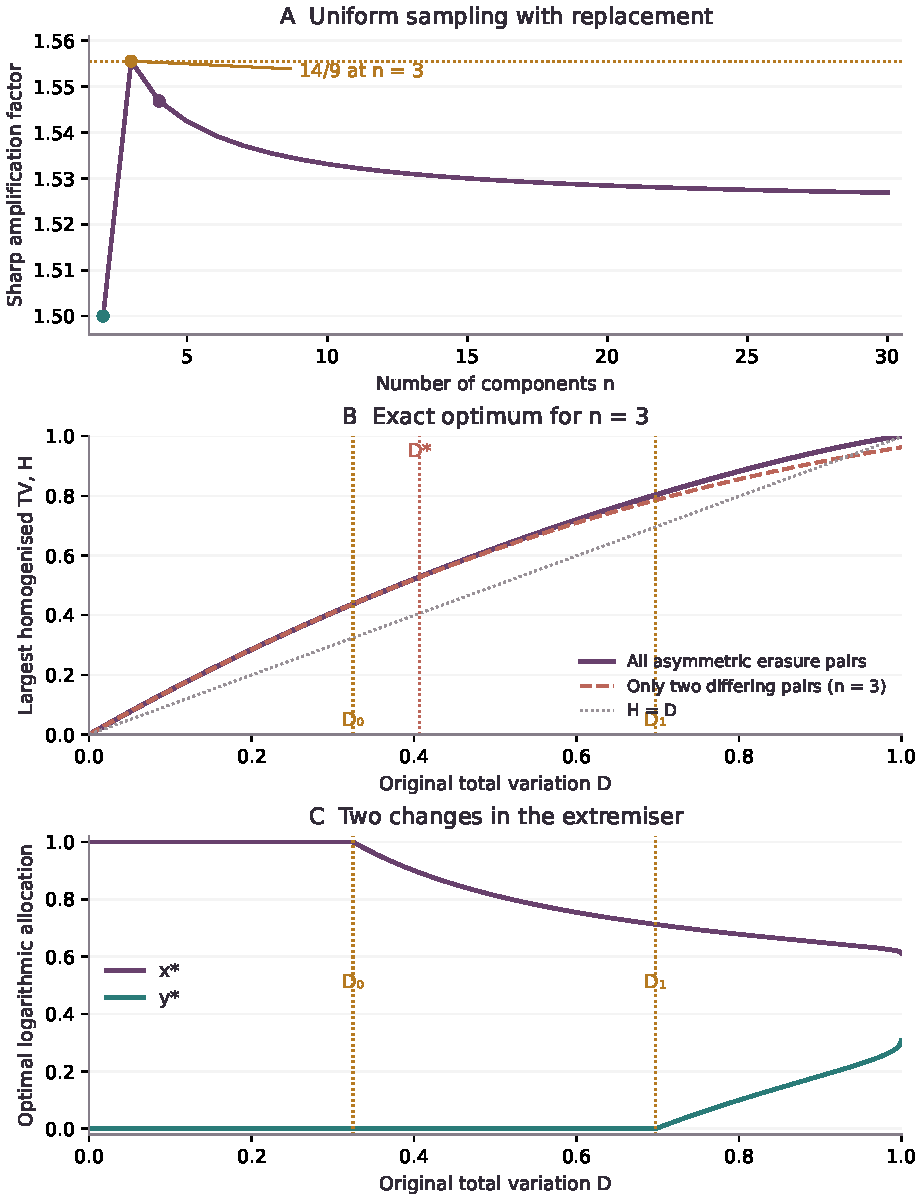
\includegraphics[width=\textwidth]{figures/sharp_homogenisation.pdf}
\caption{A: the sharp factors $C_n$ for uniform resampling of $n$ erasure experiments; the maximum $14/9$ is at $n=3$. B: the exact three-component erasure optimum $\mathcal H_3$ (Theorem~\ref{thm:three}) and the two-differing-coordinate curve $F_3$ (Theorem~\ref{thm:twoactive}); dotted lines mark the transitions $D_0,D_1$ and the crossover $D_*$ of \eqref{eq:envelope}, where $F_2$ (not plotted) overtakes $F_3$. C: the optimal logarithmic allocations $x^*,y^*$. All curves are evaluations of proved formulas.}
\end{figure}

\subsection{The general constant: a conjecture and evidence}
Combining \eqref{eq:fourteen} with \cite{KApr}, the best general constant satisfies $0.1489<c^*\le9/14$.
\begin{conjecture}\label{conj:914}
$c^*=9/14$: for all $n$ and all pairs of probability measures, $\TV(\bar P^{\otimes n},\bar Q^{\otimes n})\le\frac{14}{9}\TV(\bigotimes_iP_i,\bigotimes_iQ_i)$.
\end{conjecture}
Evidence. We maximised the labelled ratio $H_\nu/D$, which is at least $H/D$, under uniform resampling over arbitrary experiments on $m$-point outcome spaces, using 40 random restarts of a derivative-free optimiser for each $(n,m)\in\{(2,2),(2,3),(3,2),(3,3),(3,4),(4,2)\}$. The largest values found agreed with $C_2=3/2$, $C_3=14/9$ and $C_4=99/64$ to six decimal places and never exceeded them beyond the numerical tolerance $10^{-6}$. Without labels on a common two-point space the best ratio found for $n=2$ was $1.12495$, close to the Bernoulli value $9/8$ of \cite{KJan}; on a common three-point space with $n=3$ it was $1.436$, below $14/9$. This is a finite numerical search, not a proof. Remark~\ref{rem:labelled} shows that a proof of Conjecture~\ref{conj:914} by the labelled route would itself have to be sharp at $14/9$.

\subsection{Why the erasure class is not a reduction}
Two natural ways to transfer the erasure results to arbitrary experiments fail. First, a garbling (a Markov kernel applied to the observations, the same under both hypotheses) preserves mutual absolute continuity: if $P\ll Q\ll P$ then $PK\ll QK\ll PK$. An erasure experiment with mutually absolutely continuous laws has no private regions, so $r_i=s_i=1$ and its two laws coincide. Hence an informative experiment with mutually absolutely continuous laws cannot be garbled into an informative erasure experiment. Second, revealing the maximal common part of each pair refines it into a symmetric erasure experiment with common mass $1-d_i$, where $d_i=\TV(P_i,Q_i)$; for that refinement the arithmetic--geometric mean inequality gives
\[
H'=1-\Bigl(\frac1n\sum_i(1-d_i)\Bigr)^n\le1-\prod_i(1-d_i)=D',
\]
so the refinement can never show amplification. Kontorovich's Bernoulli family $p=(1-2\epsilon,\frac12)$, $q=(1,\frac12+\epsilon)$ \cite[remarks after Theorem~1.5]{KJan}, at $\epsilon=1/10$, illustrates the loss: it has $D=1/5$, $H=87/400$ and $H/D=87/80$, while its common-part refinement has $D'=7/25$, $H'=111/400$ and $H'/D'=111/112$. These obstructions do not exclude a different extremal-replacement argument. The overlap formula \eqref{eq:overlap} is exactly where the restriction to one finite likelihood-ratio value enters; controlling nonconstant likelihood ratios on the common support is the missing step.

\subsection{Open problems}
\begin{enumerate}[leftmargin=*]
\item Prove or refute Conjecture~\ref{conj:914}, even for $n=3$ or in the limit $D\to0$.
\item Determine the Bernoulli constant (conjecturally $8/9$ \cite{KJan}).
\item Find the exact finite-distance optimum for four or more erasure experiments, and for three or more arbitrary experiments.
\item Find the leading behaviour for budgets that are not multiples of $n$, the next-order term in Theorem~\ref{thm:strongall} for arbitrary experiments, and the exact rate when $q_\nu=0$.
\item Extend Theorem~\ref{thm:schedule} to the hockey-stick divergences of differential privacy, where it would give exact amplification factors for resampling with several differing records, and to adaptive schedules.
\end{enumerate}

\paragraph{Computations.} Exact rational arithmetic was used to check the constructions directly over finite product spaces: the families \eqref{eq:five} for $n=2,\ldots,5$ at five distances; $C_n$ for $n\le40$ and its limit; the identities for $F_2$, $F_3$ and $D_*$; the three-component formula against independent constrained optimisation at nine distances and against 4916 rational chamber cases; the family \eqref{eq:radixfamily} for nine choices of $(n,k,B)$, together with the base-$B$ separation over all count vectors for $n\le5$, $k\le3$ and every $B$ from $k+1$ to $kn+1$; and the Bernoulli example. The numerical search above uses fixed seeds. These checks test the formulas and constructions; the general statements rest on the proofs.

\paragraph{AI-use statement.} This paper was prepared with substantial assistance from AI systems, which were used to develop and check the proofs, run the computations, search the literature and draft the text. Assurance consists of internal AI-assisted review and the computational checks described above; the paper has not been peer reviewed. The literature search covered the cited homogenisation, sampling and privacy-amplification papers together with keyword and formula searches; an equivalent earlier statement elsewhere cannot be excluded.

\begin{thebibliography}{9}
\bibitem{BBG} Balle, B., Barthe, G., \& Gaboardi, M. (2018). \emph{Privacy amplification by subsampling: Tight analyses via couplings and divergences} (arXiv:1807.01647v2). \url{https://arxiv.org/abs/1807.01647}.
\bibitem{Sampling} Darroch, J. N., Jirina, M., \& Speed, T. P. (1988). Sampling without replacement: Approximation to the probability distribution. \emph{Journal of the Australian Mathematical Society. Series A, 44}(2), 197--213. \url{https://doi.org/10.1017/S1446788700029785}.
\bibitem{KTen} Kontorovich, A. (2025). On the tensorization of the variational distance. \emph{Electronic Communications in Probability, 30}, 1--10. \url{https://doi.org/10.1214/25-ECP680}.
\bibitem{KJan} Kontorovich, A. (2026a). \emph{TV homogenization inequalities} (arXiv:2601.04079v3). \url{https://arxiv.org/abs/2601.04079}.
\bibitem{KApr} Kontorovich, A. (2026b). \emph{A homogenization principle for total variation} (arXiv:2604.03882v1). \url{https://arxiv.org/abs/2604.03882}.
\bibitem{KOct} Kontorovich, A. (2026c). \emph{A local-to-global principle for $f$-divergence homogenization} (arXiv:2610.31164v1). \url{https://arxiv.org/abs/2610.31164}.
\end{thebibliography}
\end{document}
